\documentclass[22pt]{beamer}
\usepackage[orientation=portrait, size=custom, width=91.44, height=91.44,scale=1.2]{beamerposter} % 36in*2.5 = 90cm
\usepackage[absolute,overlay]{textpos}
\usepackage{bookmark} %pdflatex says to use this to avoid errors...
\usepackage{graphicx} %for including images
\graphicspath{{figs/}} %location of images
\usepackage{wrapfig} %wrap text around the images
\usepackage{listingsutf8}    %package for code environment; use this instead of verbatim to get automatic line break; use this instead of listings to get (•)
\usepackage{amsmath}
\usepackage{gensymb}
\usepackage[export]{adjustbox}
\usepackage[skins,theorems]{tcolorbox}
\usepackage{tikz}
\newcommand*\circled[1]{\tikz[baseline=(char.base)]{
            \node[shape=circle,draw,inner sep=2pt] (char) {#1};}}
\usepackage{array}
\usepackage{booktabs,adjustbox}
\usepackage{subcaption}
\usepackage{pgfplots}
%plot options
\pgfplotsset{width=7cm,compat=1.8}
\PassOptionsToPackage{gray}{xcolor}

\usetikzlibrary{shapes,shapes.geometric,arrows,fit,calc,positioning,automata,}

\usepackage{wrapfig}

%\mode<presentation>
%this doesn't seem to make any difference; leave for now for trying out
\usetheme{Berlin}
\definecolor{MacBlue}{rgb}{0.10196,0.22353,0.53725}
\definecolor{MacMaroon} {rgb}{0.47843, 0, 0.23137}
\definecolor{MacMaroon2} {rgb}{0.47451, 0, 0}
\definecolor{MacGray}{rgb}{0.50196,0.49804,0.51765}
\definecolor{MacMaroon3}{rgb}{00.47,0.2,0.31}
\definecolor{MacGold}{rgb}{1, 0.75,0.35}
\usecolortheme[named=MacMaroon2]{structure}
\setbeamertemplate{caption}[numbered]
\setbeamertemplate{navigation symbols}{}

\title{Pillbox: Bringing Patient Experiences into the 21st Century}
\subtitle{}  %probably want a better subtitle
  \author[Santana, Santana, Khan \& Khedri]{Carlos Santana, Cesar Santana, Madeeha Khan, Ridha Khedri$^\dagger$ \vspace{0.3cm} \newline \small \{khanm57, santanca, santanjc\}@mcmaster.ca}
  \institute[McMaster University]{$^\dagger$Department of Computing and Software, McMaster University}
  \date{December 5, 2018}

\begin{document}
%compile with pdflatex

%there is only one frame, because there is only one page; yeah, it's a poster
%textblock and block seem to work nicely to organize layout
\begin{frame}[fragile]

\begin{textblock}{2}(0.7,1)

\includegraphics[height=8.5cm]{englogo.png} % We can use CAS logo as well?
\end{textblock}

\begin{textblock}{2}(12.1,1)

\includegraphics[height=7cm, width=20cm]{pillbox_logo.png}
\end{textblock}

\begin{textblock}{8}(4,1)
\titlepage
\end{textblock}

\begin{textblock}{7.25}(0.5,2.45)
\begin{document}
%•
\end{document}\begin{block}{Introduction}
The idea behind Pillbox is to build an application which will help patients and pharmacists better keep track of medication dispensary and usage. The application is mainly geared towards patients, and will serve a wide range of users, including the elderly and children. \\
Nowadays, pharmacies have high-tech methods of dispensing, counting, and keeping track of medications and prescriptions. However, the user experience for patients has remained stagnant. Patients still need to count their own remaining medication, set various alarms, and set their own reminders to get prescriptions for important drugs refilled. The model of the traditional pill organizer was the inspiration for this project, and will be largely featured in the application, to make the app a familiar landscape and make it more intuitive for users.\\
Pillbox will use the latest technology available to make the patient experience as secure, efficient, and user-friendly as possible.
\end{block}

\begin{block}{Inspiration: Jigsaw Teaching Framework}
Jigsaw provides a social learning framework. It was introduced in 1971 by Dr. Elliot Aronson to defuse hostility and distrust between students after the desegregation of public schools in the US \cite{aronson2002building}.

The jigsaw teaching technique mainly consists of:
\begin{enumerate}
    \item Dividing subject material into segments and creating groups of the same size,
    \item Assigning one segment to each student and having them become experts in it,
    \item Have students present their segments to each other,
    \item Finally, test students on all segments of the subject material.
\end{enumerate}

Many studies have shown that students using the jigsaw teaching technique had higher levels of self-esteem, performed better on standardized exams, enjoyed school more, and worked together better than in traditional classroom settings.

\end{block}

\begin{block}{Target}
The target audience of the application are people who use medication regularly. It is directed especially to those who experience chronic illnesses, the elderly and/or anyone who may need assistance taking medication. The goal for the application is to be easily accessible and effortless to use, as well as low in data, storage. 
\end{block}

\begin{block}{Why Pillbox is needed}
The Medisafe and MyTherapy apps have over 1 million downloads each on the Play Store. While these apps may be simple and easy to use they lack some key features that would be needed by many who use medication on a daily basis. The chart below illustrates some of these key features.

\begin{center}
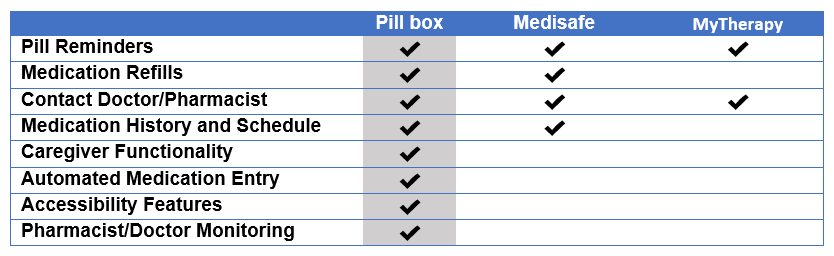
\includegraphics[height=10.5cm]{CompetitiveAdvantage.png}
\end{center}
\end{block}

\end{textblock}



\begin{textblock}{7.25}(8.25,2.9)

\begin{block}{Use Case UML Diagram}

\begin{figure}
\begin{center}
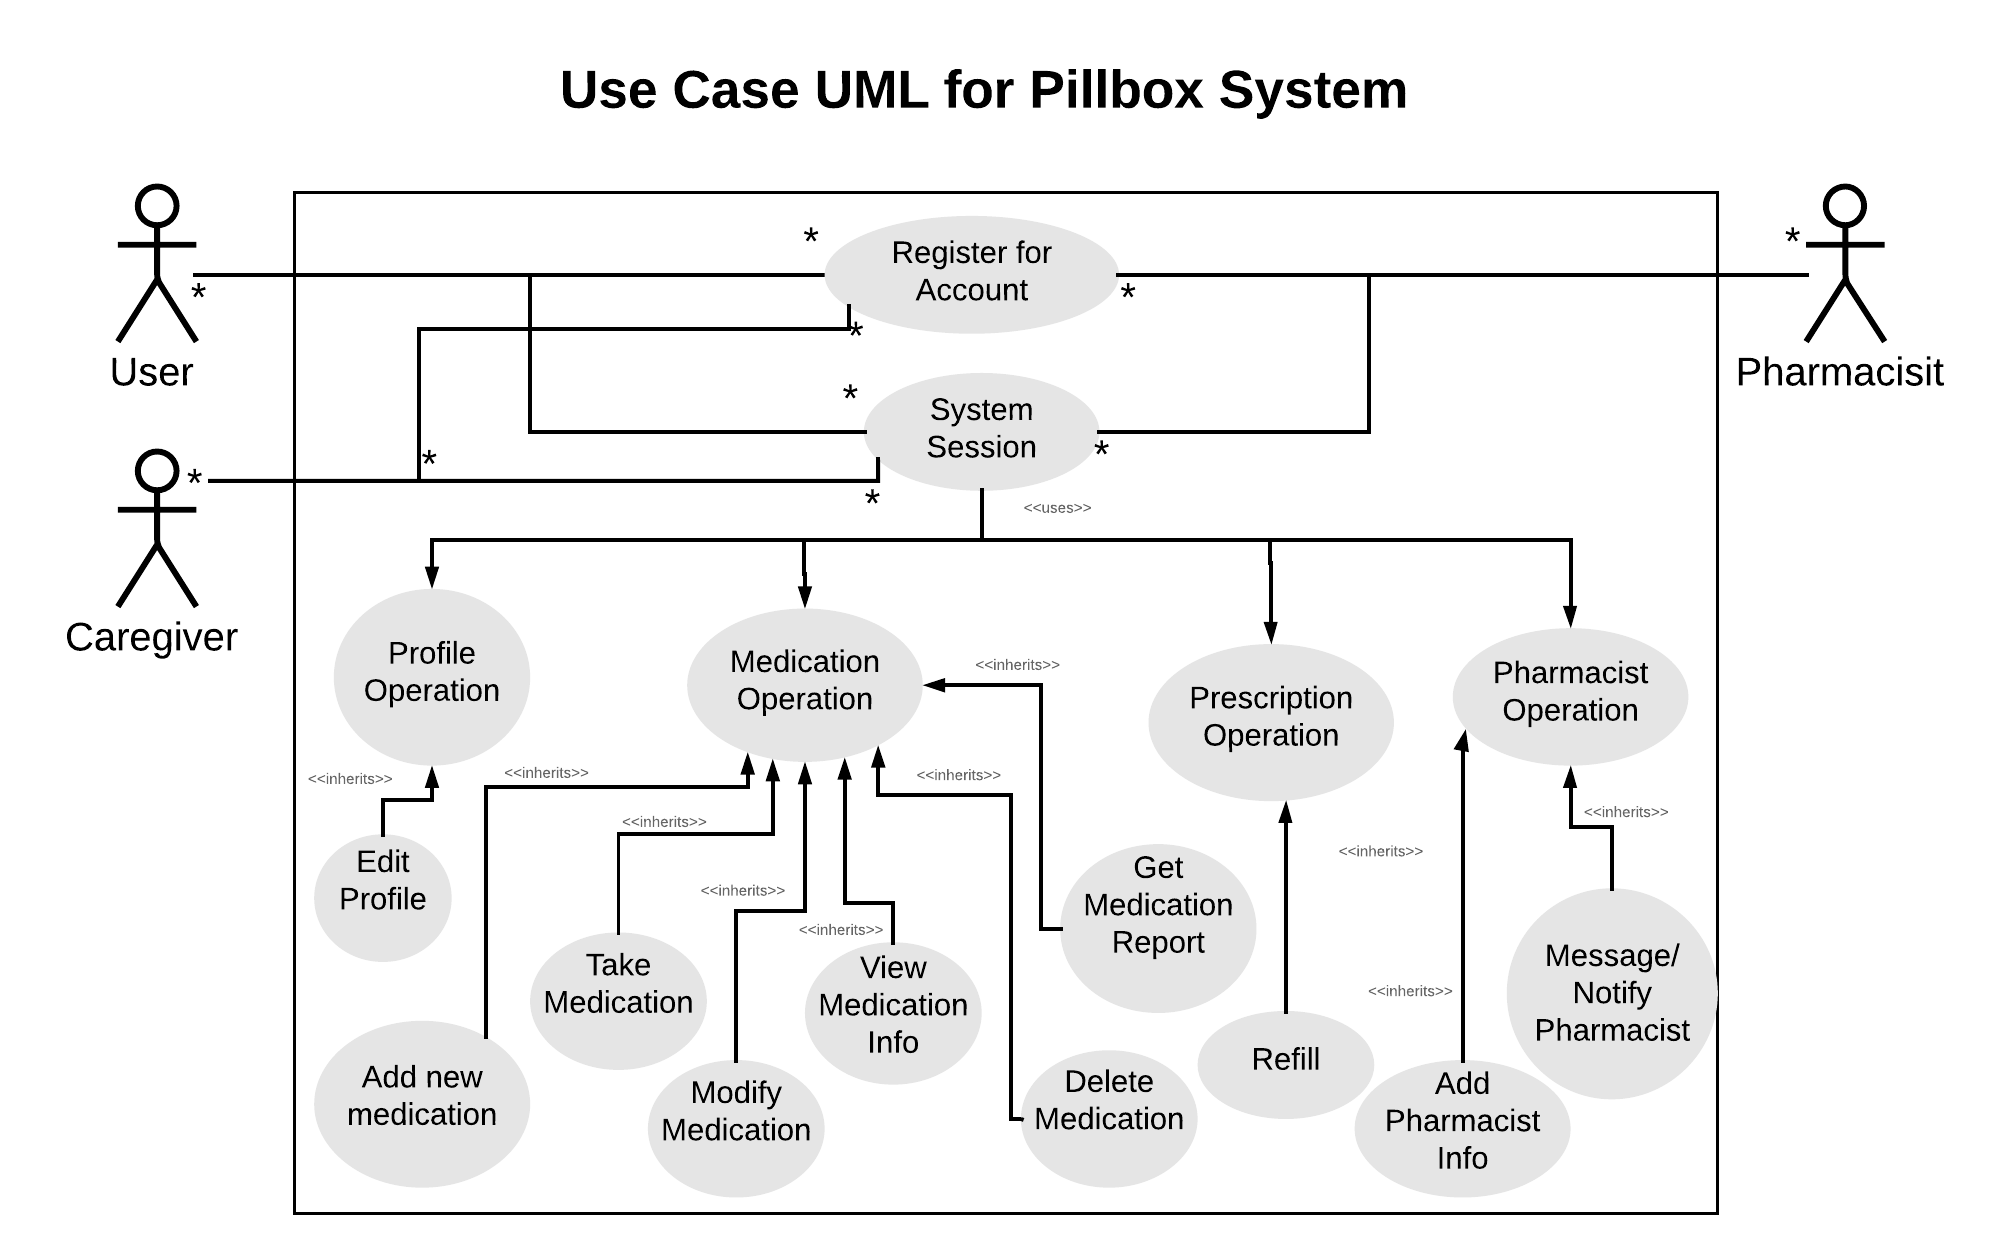
\includegraphics[height=25cm, width=40cm]{UseCaseUML.png}
\end{center}
\caption{Use Case Diagram for the Pillbox system. }
\end{figure}
The above diagram illustrates the three actors and their role with interacting with the system. An actor is a role played by one of three users: the user, the caregiver, and the pharmacist. The different actors will interact with the system to conduct a number of operations. The user role is able to view their medication information, adding new prescriptions, receive reminders to take medication and add pharmacy information.

\end{block}


\begin{block}{Conclusions \& Future Work}
The desing allows for medication users, the pharmacist, and caregivers to be involved in the medication process. Pillbox intends on sending out a survery to ensure that nothing was missed in during our requirements gathering. Pillbox is ready to start designing and implementing the solution. We intend on creating the mobile application and having it ready for testing by early 2019. There is always room to improve and adding more features is always up for discussion.

\end{block}

\begin{block}{Acknowledgements}
The Pillbox team would like to thank Dr. Kehdri for all the help and guidance he has done.
\end{block}

\begin{block}{References}
\setbeamertemplate{bibliography item}{\insertbiblabel}
\bibliographystyle{ieeetr}
{\scriptsize
\bibliography{bib}}
\end{block}

\begin{comment}
%these aren't in any particular style, it's just the basic idea
\begin{block}{References}
\setbeamertemplate{bibliography item}{\insertbiblabel}
\bibliographystyle{ieeetr}
{\scriptsize
\bibliography{bib}}
\end{block}
\vspace{-1.8mm}
%will need some more graphics to thank the various people
\end{comment}
\begin{figure}[htbp]
\centering

\includegraphics[height=5cm]{dh.png}
\hspace{1cm}

\includegraphics[height=5cm]{dh.png}
\hspace{1cm}

\includegraphics[height=5cm]{dh.png}
\hspace{1cm}

\includegraphics[height=5cm]{dh.png}
\end{figure}
\end{textblock}


\begin{textblock}{2}(8.068571428571428,13.7)

\includegraphics[height=10cm]{dh.png}
\end{textblock}
\begin{textblock}{2}(9.975714285714284,13.7)

\includegraphics[height=10cm]{dh.png}
\end{textblock}
\begin{textblock}{2}(11.882857142857143,13.7)

\includegraphics[height=10cm]{dh.png}
\end{textblock}
\begin{textblock}{2}(13.79,13.7)

\includegraphics[height=10cm]{dh.png}
\end{textblock}

\end{frame}
\end{document}
